% @Author: AnthonyKenny98
% @Date:   2020-04-08 18:12:53
% @Last Modified by:   AnthonyKenny98
% @Last Modified time: 2020-04-08 19:21:39
\begin{figure}[H]
\begin{centering}
\begin{tabular}{c}

\begin{subfigure}{\linewidth}
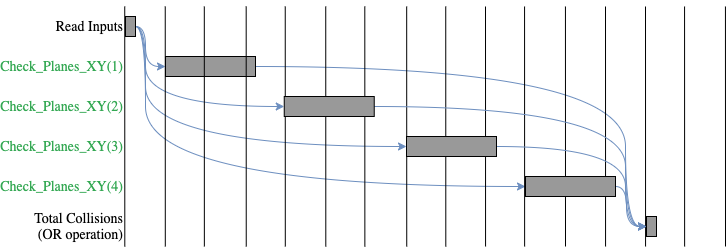
\includegraphics[width=\linewidth]{chapters/chapter3/img/timing3.png}
\caption{HoneyBee-B Timing Diagram for \texttt{Check\_Planes\_XY}. One instance of \texttt{Check\_Planes\_XY} module executed sequentially 4 times ($\epsilon=4$.}
\label{fig:hbb_timing_a}
\end{subfigure} \\

\begin{subfigure}{\linewidth}
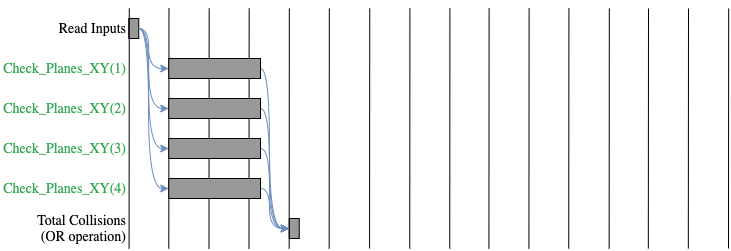
\includegraphics[width=\linewidth]{chapters/chapter3/img/timing4.png}
\caption{HoneyBee-C Timing Diagram. 4 instances of \texttt{Check\_Planes\_XY} module executing in parallel.}
\label{fig:hbb_timing_b}
\end{subfigure} \\

\end{tabular}
\mycaption{Timing Diagrams Showing Parallelization in HoneyBee-C}{. Again, these are generalizations for easy explanation of the concept of hardware parallelization. Full timing reports for each HoneyBee iteration can be found in Appendix \ref{section:honeybee_appendix_timing_reports}}
\label{fig:hbb_timing}
\end{centering}
\end{figure}